\section{Μέρος Α}
\subsection{Περιγραφή}
Στο πρώτο μέρος της εργασίας ζητήθηκε η συγκρητική αξιολόγηση μελέτη των αποτελεσμάτων τεσσάρων
ensemble αλγορίθμων ταξινόμησης. Για την εξαγωγή ορθών συμπερασμάτων ήταν απαραίτητη η δοκιμασία τους σε διαφορετικά σύνολα δεδομένων καθώς επίσης και η διενέργεια στατιστικών τεστ για την ορθή αξιολόγηση των αποτελεσμάτων. Για την υλοποίηση των παραπάνω επιλέχθηκαν τα εξής:

\begin{itemize}
	\item \textbf{Σύνολα Δεδομένων} \\
	Για την εκπόνηση του πρώτου μέρους της εργασίας επιλέχθηκαν δέκα σύνολα δεδομένων κειμένου
	τα οποία είχαν παρεμφερές περιεχόμενο και οι εγγραφές τους κατηγοριοποιούταν σε δύο κλάσεις της μορφής spam/ham, deceptive/truthfull κλπ. 
	
	Τα γνωρισμάτα που χρησιμοποιήθηκαν ήταν βασικές μετρικές όπως ο αριθμός των λέξεων, ο αριθμός των συλλαβών, δείκτες αναγνωσιμότητας (π.χ. flesch - kincaid, smog index), καθώς επίσης και απαριθμητές λέξεων που 
	ανήκουν σε συγκεκριμένες κατηγορίες π.χ. [senses, certainty, motion, negations κλπ.]. Το πλήθος των γνωρισμάτων που χρησιμοποιήθηκαν είναι 77. 
	
	\begin{table*}
		\centering
		\caption{Περιγραφή των Συνόλων Δεδομένων}
		\label{tab: data}
		\newcolumntype{F}{>{\centering\arraybackslash} m}
		\begin{tabular}{F{3.5cm}F{1cm}F{1.5cm}F{1.2cm}F{1.8cm}F{1.8cm}F{1.6cm}}
			\hline
			\ttfamily Dataset Name & \ttfamily Abbr. & \ttfamily Repos & \ttfamily Data type & \ttfamily Classes	& \ttfamily Instances & \ttfamily Balanced \\
			\hline
			Deceptive opinion spam corpus & 1 & kaggle & text & truthfull / deceptive & 1600 & yes \\ \hline
			Ironic corpus & 2 & kaggle & text & yes / no & 1950 & yes \\ \hline
			Sentiment Labelled Sentences - Amazon & 3 & UCI & text & positive / negative & 1000 & no \\ \hline
			Sentiment Labelled Sentences - IMDB & 4 & UCI & text & positive / negative & 1000 & yes \\ \hline
			Sentiment Labelled Sentences - Yelp & 5 & UCI & text & positive / negative & 1000 & yes \\ \hline
			SMS Spam collection & 6 & UCI & text & spam / ham & 5090 & no \\ \hline
			Twitter airline sentiment & 7 & Kaggle & text & positive / negative & 11540 & no \\ \hline
			Youtube Spam Collection - KatyPerry  & 8 & UCI & text & spam / ham  & 350 & yes \\ \hline
			Youtube Spam Collection - LMFAO & 9 & UCI & text & spam / ham & 438 & yes \\ \hline
			Youtube Spam Collection - Shakira & 10 & UCI & text & spam / ham & 370 & yes \\ \hline
		\end{tabular}
	\end{table*}
	
	
	\item \textbf{Pipeline - Αλγόριθμοι} \\
	 Για την εκπόνηση των πειραμάτων ακολουθήθηκε η εξής διαδικασία: Το κάθε σύνολο δεδομένων χωρίστηκε αρχικά σε train και test set (70\% - 30\% αντίστοιχα). Στη συνέχεια, αφού τα αρχικά σύνολα κανονικοποιήθηκαν, για κάθε αλγόριθμο εκτελέστηκε ένα εκτεταμένο gridsearch με 10-fold cross validation στο train set. Το μοντέλο που προέκυψε από την παραπάνω διαδικασία αξιολογήθηκε στο test set του αρχικού συνόλου δεδομένων. 
	 
	 Δεδομένου ότι στα σύνολα που χρησιμοποιήσαμε οι δύο κλάσεις είναι κατα κύριο λόγο ισοκατανεμημένες και καθώς δεν υπάρχει κάποιο κόστος για την λανθασμένη ταξινομήση σε κάποια κλάση, θεωρήσαμε ότι η ακρίβεια (accuracy) είναι μία μετρική που μπορεί να καλύψει με επάρκεια το συγκεκριμένο θέμα.\\
	 
    Οι αλγόριθμοι που επιλέχθηκαν προς σύγκριση ήταν οι εξής: adaBoost\footnotemark, Bagging\footnotemark[\value{footnote}], GradientBoost \& RandomForest.
	\footnotetext{with Decision Tree as an estimator}\\
	 
\end{itemize}

\subsection{Αποτελέσματα}
Για την καλύτερη και ευκολότερη κατανόηση των αποτελεσμάτων της πειραματικής διαδικασία, αποφασίσθηκε
η οπτικοποίησή τους σε διάφορα επίπεδα. Συγκεκριμένα εκτυπώθηκαν boxplots μετ τα αποτελέσματα του cross validation, οι καμπύλες μάθησης (learning curves), καθώς επίσης και το διάγραμμα για την εύρεση των στατιστικά σημαντικών διαφορών στις αποδόσεις των αλγορίθμων (CD diagram). Επιπλέον, σε αυτή την ενότητα θα γίνει και ο σχολιασμός των αποτελεσμάτων. 

\subsubsection{Boxplots}
Για την παρακολούθηση της επιλογής παραμέτρων για τον κάθε αλγόριθμο και για κάθε σύνολο δεδομένων, αποφασίσθηκε η εκτύπωση των αποτελεσμάτων του μοντέλου με την καλύτερη απόδοση για το συνόλο των test results εντός του 10 fold cross validation με την μορφή Boxplots. Επιπλέον, το συγκεκριμένο γράφημα συνοδεύται από την εκτύπωση (σε μορφή barchart) των αποτελεσμάτων του βέλτιστου μοντέλου στο test set που είχε αρχικά αποκλειστεί από την διαδικασία μάθησης. Τα αποτελέσματα φαίνονται στον πίνακα \ref{tab:boxplots}. Εύκολα μπορούμε να διαπιστώσουμε
ότι γενικά δεν έχουμε καλή συμπεριφορά των μοντέλων στην πλειοψηφία των συνόλων δεδομένων με εξαίρεση ίσως στα σύνολα 6 \& 7.

\begin{table*}
	\centering
	\caption{Αποτελέσματα από την εκπαίδευση των αλγορίθμων και από την αξιολόγησή τους στο test set του κάθε συνόλου δεδομένων.}
	\label{tab:boxplots}
	\begin{tabular}{cc}
		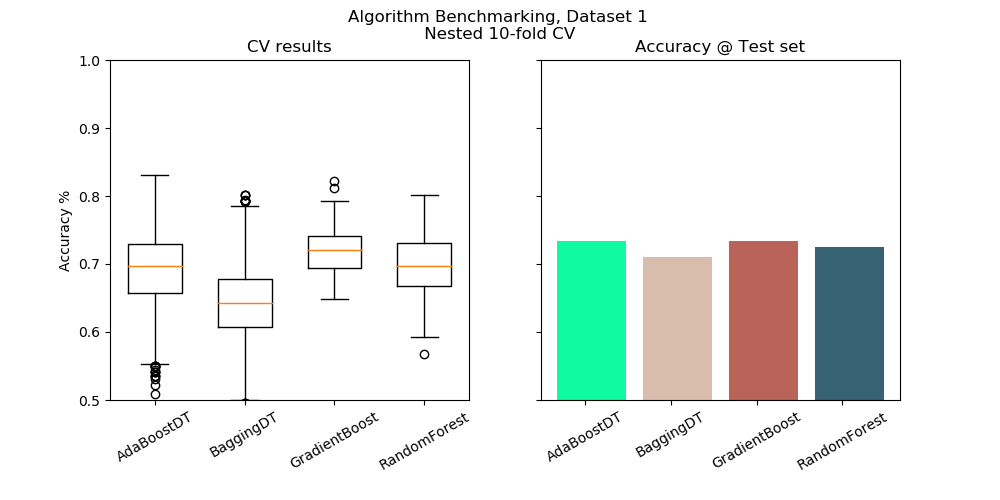
\includegraphics[width=70mm,height = 40mm]{1.png} &
		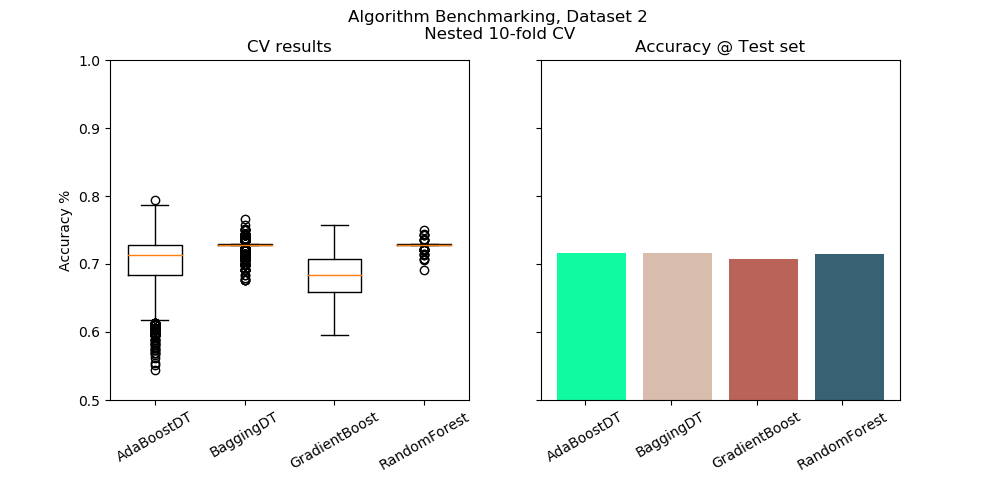
\includegraphics[width=70mm,height = 40mm]{2.png} 
		 \\ %\hline
		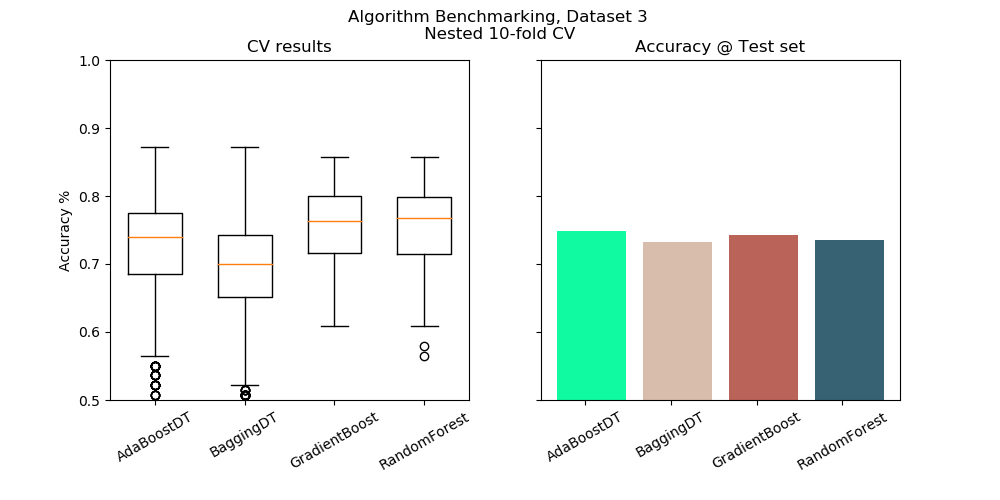
\includegraphics[width=70mm,height = 40mm]{3.png} &
		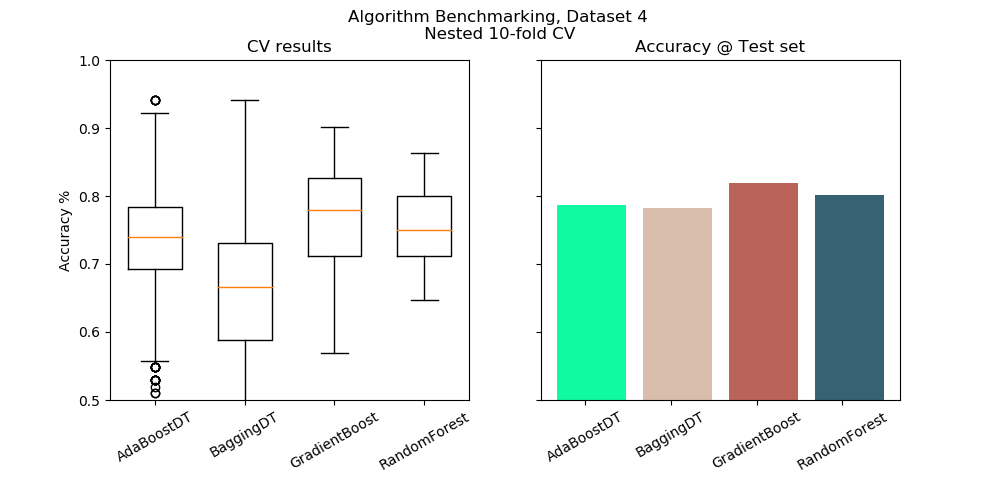
\includegraphics[width=70mm,height = 40mm]{4.png} 
		 \\ %\hline
		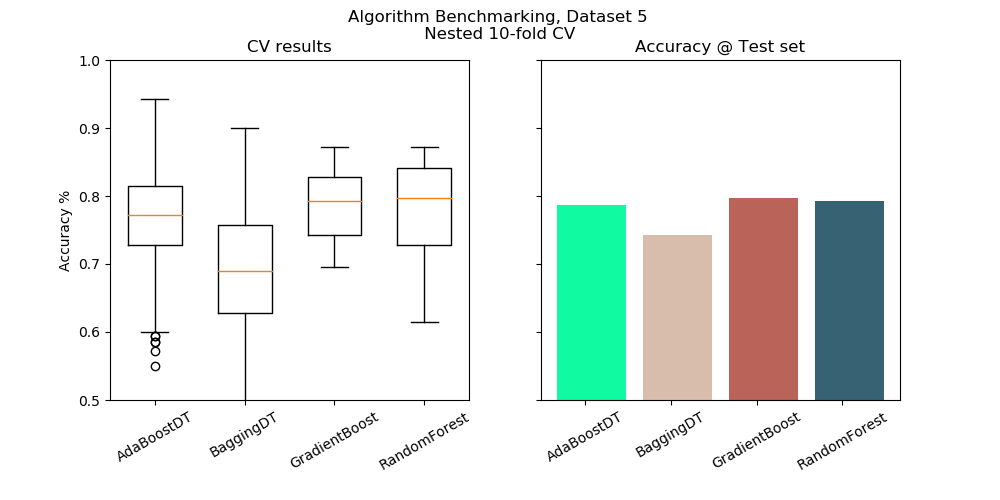
\includegraphics[width=70mm,height = 40mm]{5.png} &
		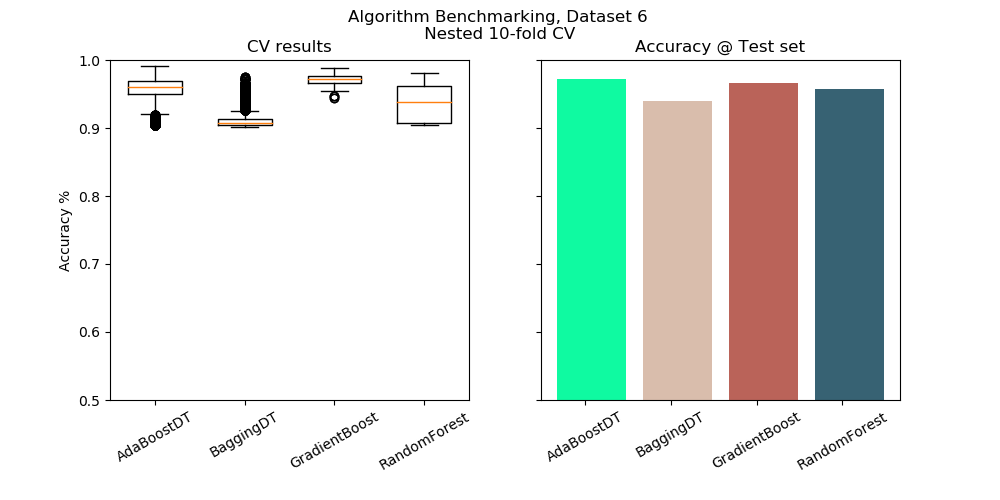
\includegraphics[width=70mm,height = 40mm]{6.png} 
		 \\ %\hline
		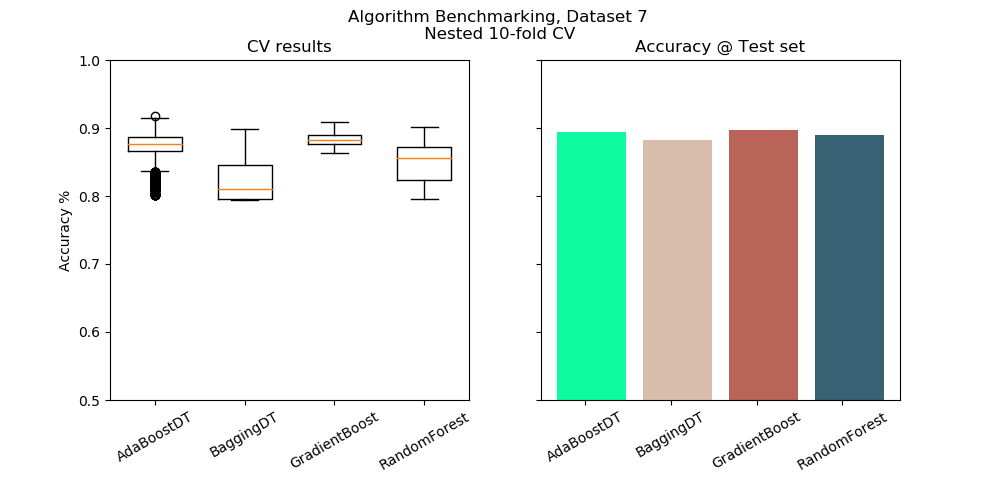
\includegraphics[width=70mm,height = 40mm]{7.png} &
		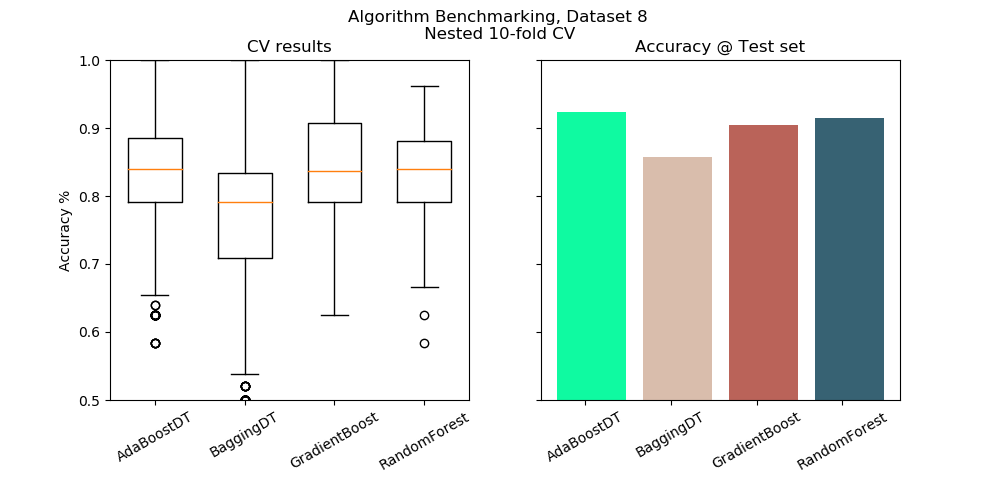
\includegraphics[width=70mm,height = 40mm]{8.png} 
		 \\ %\hline
		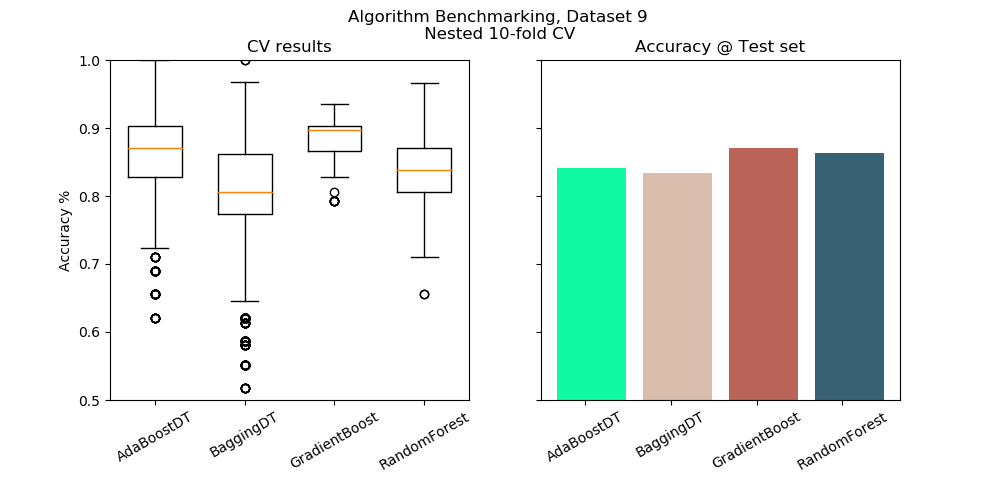
\includegraphics[width=70mm,height = 40mm]{9.png} &
		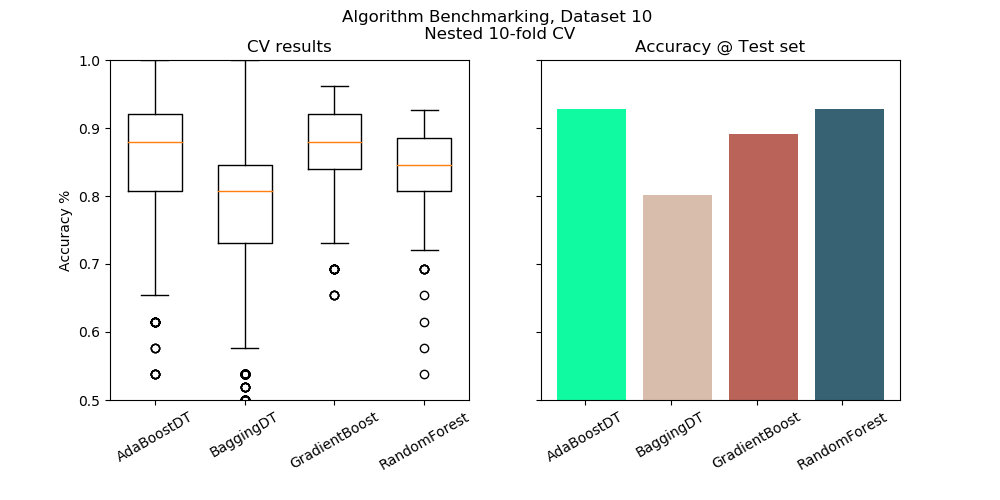
\includegraphics[width=70mm,height = 40mm]{10.png}
	\end{tabular}
\end{table*}


\subsubsection{Καμπύλες μάθησης}

Ώς συνέχεια του προηγούμενου βήματος αξιολόγησης αποφασίσθηκε και η εκτύπωση των καμπυλών μάθησης. Όπως φαίνεται και στο Σχήμα \ref{fig:learning_curves}, μετά το εκτεταμένο grid search είναι εμφανής η τάση για σφαλματώδη υπεραρμογή (overfitting) στις περισσότερες των περιπτώσεων. Αξίζει να σημειώσουμε αυτήν την παρατήρηση αλλά και επίσης ότι δεν θα ασχοληθούμε με την επίλυση του συγκεκριμένου προβλήματος στην παρούσα εργασία καθώς δεν είναι εντός των πλαισίων της.

\begin{figure}
	\centering %\textwidth
	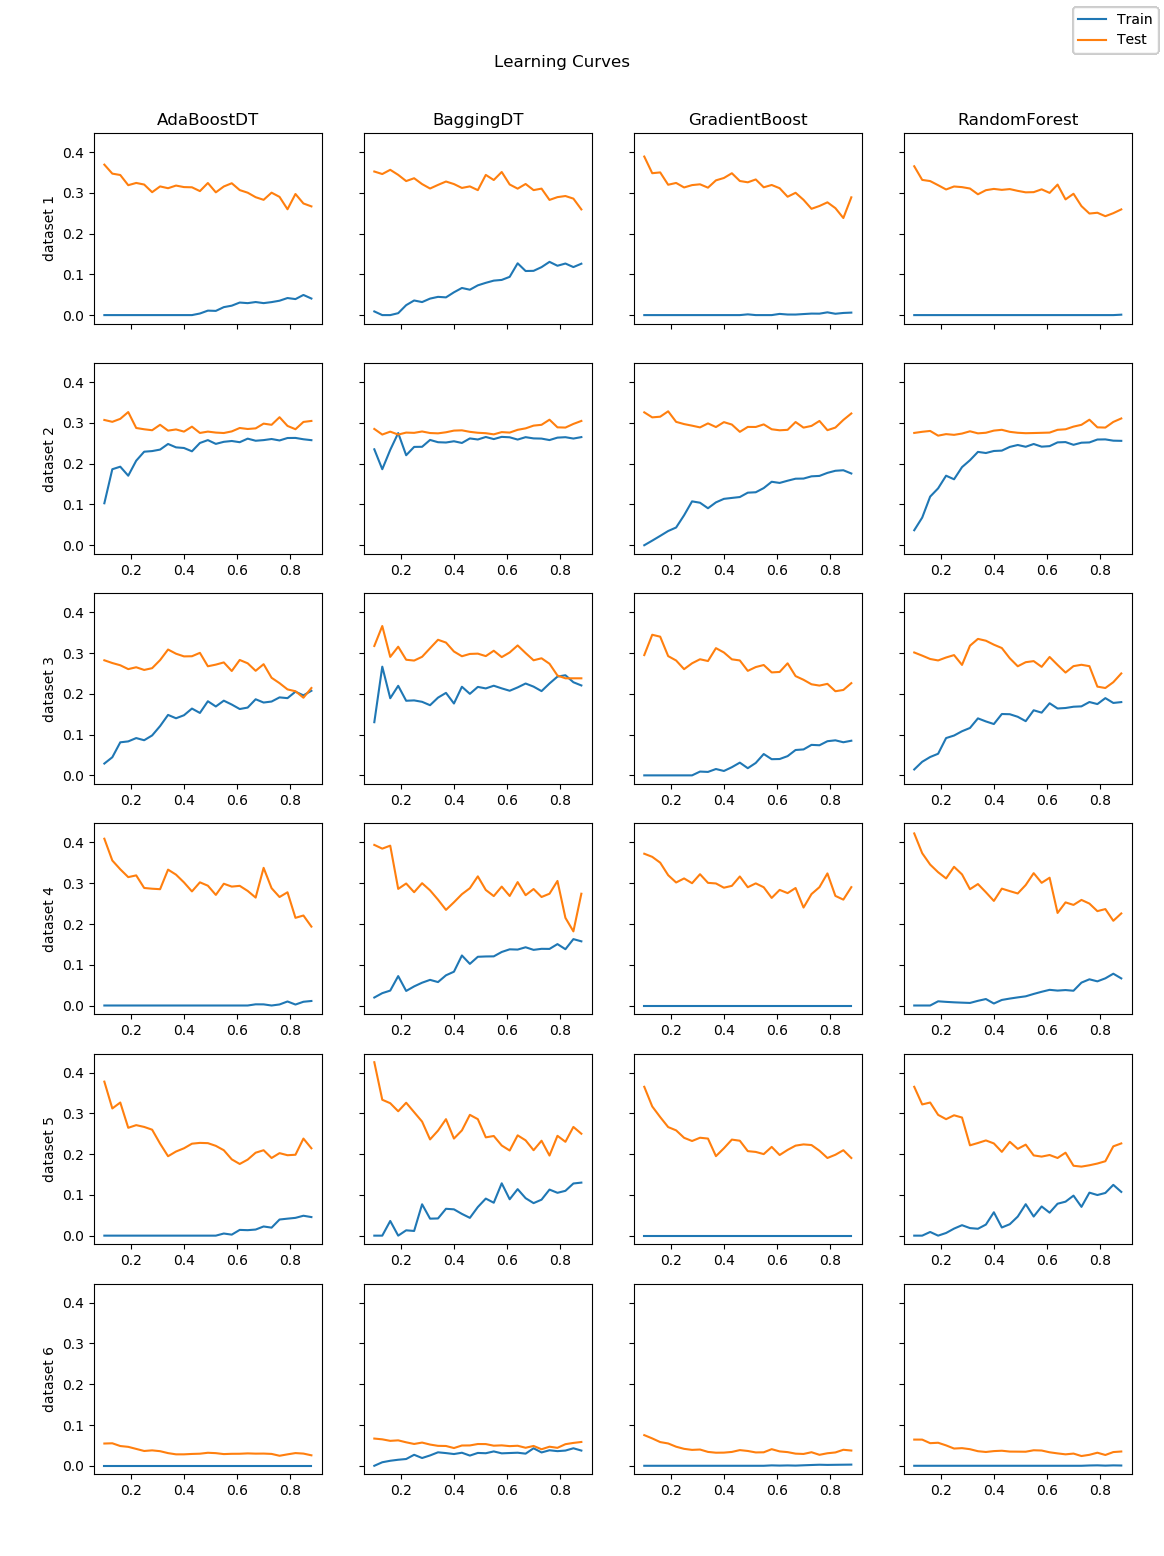
\includegraphics[scale=0.5]{learning_curves.png}
	\caption{Learning curves 1 από 2. Κάθε γράφημα απεικονίζει την καμπύλη μάθησης για κάθε σύνολο δεδομένων και για κάθε αλγόριθμο. Στο άξονα των $y$ έχουμε το σφάλμα \% ενώ στον άξονα των $x$ έχουμε το ποσοστό του συνόλου δεδομένων που έχει χρησιμποιηθεί για την εκπαίδευση και την αξιολόγηση του κάθε μοντέλου. Το βήμα που έχει χρησιμοποιηθεί για την κατανομή σε μέρη είναι το 3\% του κάθε συνόλου.}
	\label{fig:learning_curves}
\end{figure}

\begin{figure}
	\centering %\textwidth
	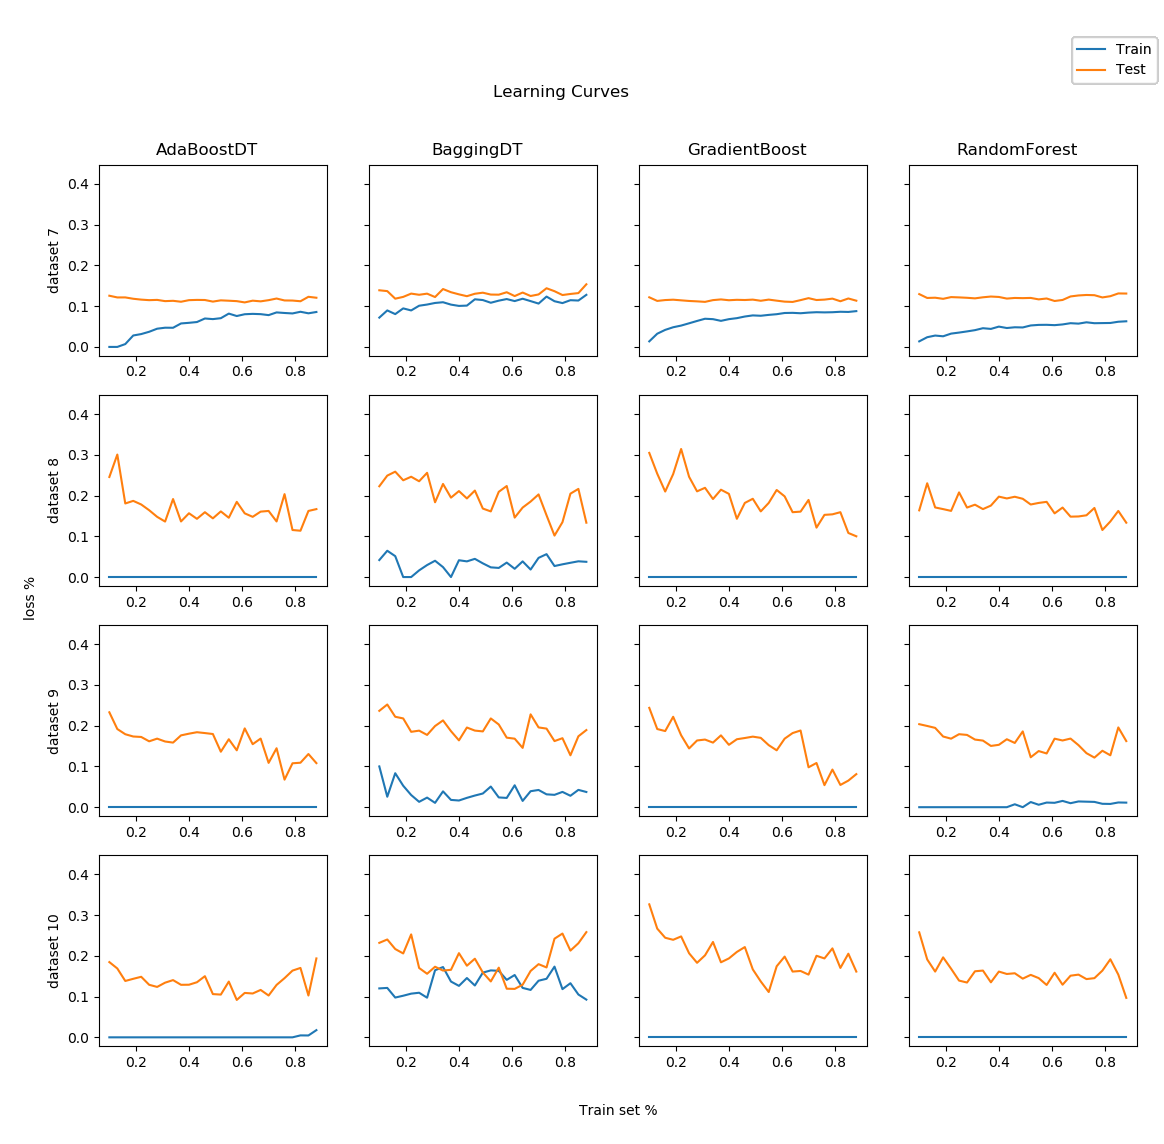
\includegraphics[scale=0.5]{learning_curves2.png}
	\caption{Learning curves 2 από 2. Κάθε γράφημα απεικονίζει την καμπύλη μάθησης για κάθε σύνολο δεδομένων και για κάθε αλγόριθμο. Στο άξονα των $y$ έχουμε το σφάλμα \% ενώ στον άξονα των $x$ έχουμε το ποσοστό του συνόλου δεδομένων που έχει χρησιμποιηθεί για την εκπαίδευση και την αξιολόγηση του κάθε μοντέλου. Το βήμα που έχει χρησιμοποιηθεί για την κατανομή σε μέρη είναι το 3\% του κάθε συνόλου.}
	\label{fig:learning_curves2}
\end{figure}


\subsubsection{Συγκριτική αξιολόγηση -  Friedman test}

Για την αξιολόγηση των αλγορίθμων όπως έχουμε αναφέρει ήδη επιλέχθηκε η μετρική της ακρίβειας (accuracy).
 Με το πέρας των πειραμάτων και για την τελική αξιολόγηση της κατάταξης των αλγορίθμων, 
 επιλέχθηκε η μέθοδος Friedman για την εύρεση ή μη στατιστικά σημαντικών διαφορών. 
 Όπως αναφέρει ο \citet{demvsar} για για την εκτέλεση του εξελιγμένου Friedman test όπως 
 το πρότειναν οι \citet{iman1980}, αρχικά θα πρέπει να δημιουργηθεί 
 ο Πίνακας κατάταξης (βλ. Πίνακα \ref{tab:ranking}) και στη συνέχεια να υπολογιστούν οι εξής τιμές:

\begin{equation}
\label{eq:X_def}
	x_F^2 = \frac{12N}{k(k+1)}\Big[ \sum_{j}R_j^2 - \frac{k(k+1)^2}{4} \Big]  
\end{equation}
\begin{equation}
\label{eq:F_def}
	F_F = \frac{(N −1)x_F^2}{N(k-1)-x_F^2}
\end{equation}

Σε περίπτωση που το αποτέλεσμα της εξίσωσης 2 είναι μεγαλύτερο από την τιμή της κατανομής όπως ορίζεται 
από τον πίνακα κατανομής \emph{F-distribution}, τότε θα πρέπει να συνεχίσουμε με το post hoc test
 για το οποίο θα πρέπει να υπολογίσουμε την τιμή \emph{CD}.

\begin{equation}
\label{eq:CD_def}
	CD = q_a\sqrt{\frac{k(k+1)}{6N}}
\end{equation}


Πράγματι, αν εφαρμόσουμε τις τιμές του Πίνακα \ref{tab:ranking} στις εξισώσεις 
\ref{eq:X_def} \& \ref{eq:F_def} για το συγκεκριμένο πρόβλημα της εργασίας θα έχουμε τα παρακάτω αποτελέσματα

\begin{equation}
\label{eq:X_value}
x_F^2 = \frac{12\cdot 10}{4\cdot(4+1)}\Big[ (1.85^2+3.75^2+1.95^2+2.55^2) - \frac{4\cdot(4+1)^2}{4} \Big]  = 16.74
\end{equation}

\begin{equation}
\label{eq:F_value}
F_F = \frac{9 \cdot 16.74}{30 - 16.74} = 11.36
\end{equation}

Επειδή η τιμή που προκύπτει από την \ref{eq:F_value} είναι μεγαλύτερο από το \emph{$F_{3,27} = 2.96$}, απορίπτουμε την παραδοχή ότι δεν υπάρχει στατιστικά σημαντική διαφορά στην κατάταξη των αλγορίθμων και συνεχίζουμε στον υπολογισμό της τιμής $CD$ όπως φαίνεται στην εξίσωση \ref{eq:CD_value}.

\begin{equation}
\label{eq:CD_value}
CD = 2.569\sqrt{\frac{4\cdot 5}{6 \cdot 10}} = 1.4832
\end{equation}

\begin{table*}
	\centering
	\caption{Αποτελέσματα και κατάταξη αλγορίθμων}
	\label{tab:ranking}
	\begin{tabular}{ccccc}
		\hline
		\ttfamily Dataset & \ttfamily AdaBoost & \ttfamily Bagginng & \ttfamily GradBoost & \ttfamily RandForest
		\\	\hline
		1&	0.733 (1.5)&    0.710 (4.0) &	0.733 (1.5)&	0.725 (3.0) \\ \hline
		2&	0.716 (1.5)&    0.716 (1.5) &	0.708 (4.0)&	0.715 (3.0)\\ \hline
		3&	0.749 (1.0)&	0.732 (4.0)&	0.742 (2.0)&	0.736 (3.0) \\ \hline
		4&	0.787 (3.0)&	0.783 (4.0)&	0.819 (1.0)&	0.801 (2.0)\\ \hline
		5&	0.787 (3.0)&	0.743 (4.0)&	0.797 (1.0)&	0.793 (2.0)\\ \hline
		6&	0.972 (1.0)&	0.940 (4.0)&	0.966 (2.0)&	0.958 (3.0)\\ \hline
		7&	0.893 (2.0)&	0.883 (4.0)&	0.897 (1.0)&	0.889 (3.0)\\ \hline
		8&	0.924 (1.0)&	0.857 (4.0)&	0.905 (3.0)&	0.914 (3.0)\\ \hline
		9&	0.841 (3.0)&	0.833 (4.0)&	0.871 (1.0)&	0.864 (2.0)\\ \hline
		10&	0.928 (1.5)&	0.802 (4.0)&	0.892 (3.0)&	0.928 (1.5)\\ \hline
		avg rank&1.85 &	3.75 & 1.95 & 2.55
		\\ \hline
	\end{tabular}
\end{table*}

Όπως φαίνεται και στο Σχήμα \ref{fig:CD} από τα αποτελέσματα της post hoc διαδικασίας βλέπουμε ότι η διαφορά μεταξύ του τελευταίου στην κατάταξη αλγορίθμου Bagging και των δύο πρώτων (AdaBoost και GradientBoost) είναι στατιστικά σημαντική. Αντιθέτως, δεν υπάρχει στατιστικά σημαντική διαφορά μεταξύ των τριών πρώτων στην κατάταξη αλγορίθμων.

\begin{figure}
	\centering
	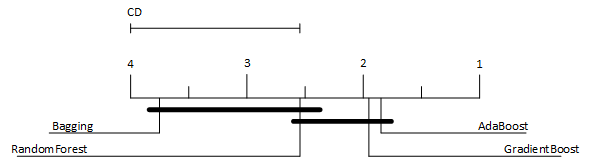
\includegraphics{CD.png} %[width=0.6\textwidth]
	\caption{Σύγκριση όλων των ταξινομητων μεταξύ τους με την χρήση του Nemenyi test. Οι ομάδες των ταξινομητών μεταξύ των οποίων δεν υπάρχει στατιστικά σημαντική διαφορά για p = 0.05 ενώνονται μεταξύ τους.}
	\label{fig:CD}
\end{figure}


\section{Μέρος Β}
Στο δεύτερο μέρος της εργασίας καλούμαστε να μελετήσουμε ένα πρόβλημα ταξινόμησης με βάση έναν συγκεκριμένο πίνακα κόστους. Συνεπώς θα πρέπει να επιτευχθεί βελτιστοποίηση των αλγορίθμων με βάση το κόστους μίας λανθασμένης ταξινόμησης και όχι κάποιας άλλης μετρικής. Θα πρέπει να σημειώσουμε εδώ ότι ενώ για το πρώτο και τρίτο μέρος της εργασίας η υλοποίηση έγινε σε Python 2.7,  δυστυχώς δεν υπάρχει κάποια ώριμη υλοποίηση για την επίλυση προβλημάτων ταξινόμησης με κριτήριο το κόστος. Γι αυτόν τον λόγο, για την υλοποίηση του Β Μέρους επιλέχθηκε το Weka. Ως συνέπεια αυτού, δυστυχώς η απεικόνιση των αποτελεσμάτων θα είναι πιο φτωχή σε σχέση με τα υπόλοιπα μέρη της εργασίας.


\subsection{Γενικά}
Όπως περιγράφεται στην εκφώνηση της εργασίας, στο Β Μέρος ζητείται η μελέτη τριών αλγορίθμων ταξινόμησης (Naive Bayes, SVM με γραμμικό πυρήνα και Random Forest) σε συνδυασμό με τεχνικές που βελτιώνουν την μάθηση σε σχέση με έναν δωθέντα πίνακα κόστους. Η σύγκριση που θα γίνει περιλαμβάνει αρχικά την ταξινόμηση χωρίς εφαρμογή αυτών των τεχνικών για την αποτύπωση μίας αρχικής κατάστασης και στη συνέχεια την εφαρμογή του MetaCost  και του CostSensitive Classifier όπως έχουν προταθεί από τους \citep{metacost} και \citep{costsensitive} αντίστοιχα. 

\subsection{Αποτέλεσματα}
Παρατηρώντας τον πίνακα αποτελεσμάτων (Πίνακας \ref{tab:cost}) μπορούμε εύκολα να συμπεράνουμε ότι για το συγκεκριμένο πρόβλημα, η επιλογή της μεθόδου MetaCost σε συνδυασμό με τον αλγόριθμο ταξινόμησης Naive Bayes οδηγεί στην ταξινόμηση των αποτελεσμάτων με το μικρότερο δυνατό κόστος. Στην προκειμένη περίπτωση αν και ουσιασικά η παρατήρηση είναι χωρίς αξία, θα πρέπει να αναφέρουμε ότι ο συγκεκριμένος συνδυασμός επιτυγχάνει και την μεγαλύτερη ακρίβεια ταξινόμησης (accuracy). Παρατηρούμε επίσης ότι οι αλγόριθμοι Naive Bayes και Linear SVM αντιμετωπίζουν το πρόβλημα με σεβασμό και στις δύο κλάσεις, ενώ ο Random Forest προκειμένου να αποφύγει την αύξηση του κόστους μειώνει στο ελάχιστο τα αποτελέσματα που κατηγοριοποιεί στην κλάση 0 χωρίς αυτό να αποτελεί καλή επιλογή. 


\begin{table}[]
	\centering
	\caption{Αποτελέσματα εφαρμογής μεθόδων μείωσης κόστους στους ταξινομητές. Για κάθε Αλγόριθμο ταξινόμησης δίνεται ο πίνακας ταξινόμησης, το κόστος ταξινόμησης σύμφωνα με τον πίνακα κόστους που έχει δοθεί καθώς επίσης και η ακρίβεια ταξινόμησης.}
	\label{tab:cost}
	\begin{tabular}{|c|ll|ll|ll|}
	\hline
	Τεχνική & \multicolumn{2}{l|}{Naive Bayes} & \multicolumn{2}{l|}{Linear SVM} & \multicolumn{2}{l|}{Random Forest} \\ \hline
	\multirow{3}{*}{Plain} & \multicolumn{1}{c}{125} & \multicolumn{1}{c|}{25} & 120 & 30 & 119 & 31 \\
	& \multicolumn{1}{c}{31}  & \multicolumn{1}{c|}{89} & 31  & 89 & 50 & 70 \\ \cline{2-7} 
	& \multicolumn{1}{c}{180} & 79.3\% & 185 & 77.4\%   & 281 & 70\% \\ \hline
	\multirow{3}{*}{MetaCost} & 110    & 40  & 105      & 45  & 10 & 140 \\
						  	  & 15     & 105 & 18       & 102 & 3  & 117              \\ \cline{2-7} 
	& \textbf{115}            & 79.6\% & 135 & 76.7\%   & 155 & 47\%        \\ \hline
	\multirow{3}{*}{CostSensitive} & 114                     & 36                      & 95             & 55             & 14              & 136              \\
	& 19                      & 101                     & 16             & 104            & 2               & 118              \\ \cline{2-7} 
	& 131                     & 79.6\%                    & 135            & 74\%           & 146             & 48.9\%             \\ \hline
\end{tabular}
\end{table}

\section{Μέρος Γ}
Στο τρίτο και τελευταίο μέρος της εργασίας, κληθήκαμε να μελετήσουμε τρόπους αντιμετώπισης του προβλήματος της ασυμμετρίας κλάσεων. Το πρόβλημα που θα μελετήσουμε προέρχεται από το \emph{Kaggle} και είναι το \emph{CreditCard Fraud}. Το συγκεκριμένο σύνολο δεδομένων περιγράφεται από 29 numeric γνωρίσματα καθώς επίσης και μία στήλη με τον χρόνο που έγινε η συναλλαγή. Θεωρώντας ότι το συγκεκριμένο γνώρισμα δεν μπορεί να προσφέρει κάτι ώς έχει (περισσότερο λειτουργεί σαν ID), αποφασίσθηκε η απομάκρυνσή του από την διαδικασία ταξινομήσης. Οι κλάσεις που περιγράφουν την κάθε συναλλαγή είναι δύο (Fraud or Not-Fraud). 
Η παρουσία των δύο κλάσεων στο σύνολο είναι εξαιρετικά ανισοκατανεμημένη. Συγκεκριμένα για την κλάση Fraud (1) υπάρχουν μόλις 492 καταγραφές σε σύνολο 284807 συναλλαγών (0.172\%). 
\subsection{Μέθοδοι - Πείραμα}

Για το τρίτο μέρος της εργασίας και για επίλυση του προβλήματος της ανισοκατανομής των κλάσεων επιλέχθηκαν οι παρακάτω μέθοδοι αναδιαμόρφωσης του συνόλου δεδομένων προς μελέτη - σύγκριση: 

\emph{EasyEnsemble},\\ \emph{Nearmiss} (Nearmiss1, Nearmiss2 ,Nearmiss3)  \& \\ \emph{SMOTE} (borderline1,borderline2, regular, svm)

Οι αλγόριθμοι ταξινόμησης που χρησιμοποιήθηκαν ήταν αυτοί που δόθηκαν στην εκφώνηση (Naive Bayes, Linear SVM \& RandomForest) με τις default παραμέτρους που δίνουν η scikit και η imbalance βιβλιοθήκες.

Εκτός από τα πειράματα με την διαχείρηση του πλήθους στο συνόλο των δεδομένων, εκτελέστηκαν πειράματα με το σύνολο δεδομένων ως είχε αρχικά με στόχο την δημιουργία ενός βασικού σημείου σύγκρισης για την απόδοση των μοντέλων. 

Για την αξιολόγηση των αποτελεσμάτων και επειδή συζητάμε το πρόβλημα της ανισοκατανομής, επιλέχθηκε η μετρική AUC.

Η υλοποίηση του τρίτου μέρους της εργασίας έγινε σε Python 2.7 με την χρήση των βιβλιοθηκών scikit - learn \citep{scikit-learn} καθώς επίσης και της βιβλιοθήκης imbalanced-learn όπως αυτή έχει περιγραφεί στο \citep{JMLR:v18:16-365}

\subsection{Αποτελέσματα}

Παρατηρώντας το Σχήμα \ref{fig:balance} στο οποίο αποτυπώνεται το σύνολο των αποτελεσμάτων των πειραμάτων που διεξήχθησαν, μπορούμε σχετικά εύκολα να βγάλουμε τα εξής συμπεράσματα: Οι \emph{Nearmiss1} \& \emph{Nearmiss2} μέθοδοι δεν έφεραν τα επιθυμητά αποτελέσματα μιας και πέτυχαν χαμηλότερα AUC scores σε σχέση με τα μοντέλα που εκπαιδεύτηκαν στο αρχικό σύνολο δεδομένων. Από την ομάδα των \emph{Nearmiss} εξαίρεση αποτέλεσε ο \emph{Nearmiss3} με χρήση του οποίου βλέπουμε βελτίωση στους δύο από τους τρεις αλγορίθμους που χρησιμοποιήσαμε (\emph{LinearSVM} \& \emph{RandomForest}). Σε δεύτερο επίπεδο η μέθοδος \emph{SMOTE} ανεξάρτητα από την συνάρτηση απόφασης που ακολουθήθηκε, φαίνεται να αποδίδει σταθερά καλύτερα σε σχέση με την εκπαίδευση στο αρχικό σύνολο δεδομένων. Και στις τέσσερις περιπτώσεις ο LinearSVM έφερε τα καλύτερα αποτελέσματα. Τέλος, το καλύτερο αποτελέσμα έναντι όλων έφερε η μέθοδος EasyEnsemble σε συνδυασμό με τον αλγόριθμο RandomForest.

\begin{figure}
	\centering
	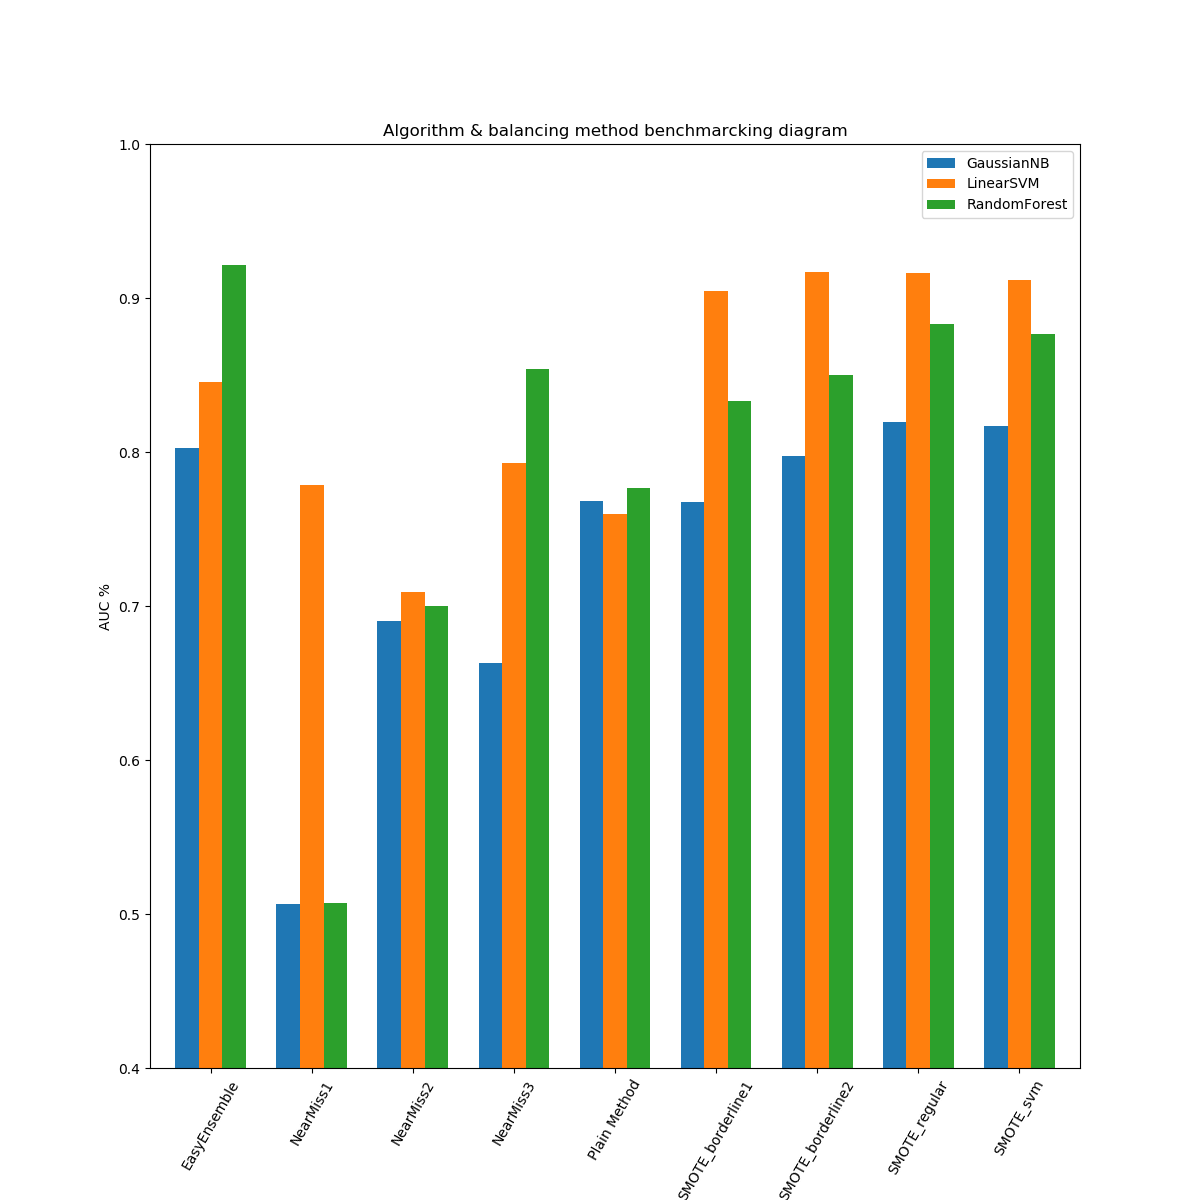
\includegraphics[width=1\textwidth]{diagram.png} %[width=0.6\textwidth]
	\caption{Σύγκριση όλων των ταξινομητών και όλων των μεθόδων διόρθωσης της ανισοκατανομής των κλάσεων μεταξύ τους.}
	\label{fig:balance}
\end{figure}

\begin{table*}
	\centering
	\caption{Απόδοση αλγορίθμων ταξινόμησης ανάλογα με την μέθοδο επίλυσης του προβλήματος της ανισοκατανομής των κλάσεων. Η μετρική που χρησιμοποιήθηκε είναι η AUC.}
	\label{tab: imbalance}
	\begin{tabular}{cccc}
			\hline
		\ttfamily Method / Algorithm & \ttfamily Naive Bayes & \ttfamily LinearSVM & \ttfamily RandomForest 	\\	\hline
		Plain Method & 0.768       & 0.760     & 0.777         \\ \hline
		NearMiss1 & 0.507       & 0.779     & 0.507\\ \hline
		NearMiss2 & 0.690       & 0.709     & 0.700\\ \hline
		NearMiss3 & 0.663       & 0.793     & 0.854\\ \hline
		EasyEnsemble & 0.803       & 0.845     & \textbf{0.921}\\ \hline
		SMOTE borderline1 & 0.768       & 0.905     & 0.833\\ \hline
		SMOTE borderline2 & 0.798       & 0.917     & 0.850\\ \hline
		SMOTE regular & 0.820       & 0.916     & 0.883\\ \hline
		SMOTE svm & 0.817       & 0.911     & 0.877\\ \hline
		

	\end{tabular}
\end{table*}


\section{Τεχνικά}

Στην ενότητα αυτή γίνεται μία σύνοψη των εργαλείων που για την εκπόνηση της εργασίας.
Γενικά, για τα περισσότερα μέρη υλοποιήθηκαν σε Python 2.7 με την χρήση διαφόρων βιβλιοθηκών
όπως η scikit-learn \citep{scikit-learn} και η imbalance-learn \citep{JMLR:v18:16-365}. Για την εξαγωγή των 
γλωσσολογικών γνωρισμάτων χρησιμοποιήθηκε το NLTK toolkit \citep{Bird:2006} και η Spacy σε συνδυασμό με την Textacy \citep{spacy} Οι κατηγορίες λέξεων προέρχονται από το LIWC \citep{LIWC}. Στα κομμάτια που δεν ήταν δυνατή η χρήση της Python χρησιμοποιήθηκε το Weka. Το σύνολο της εργασίας (κώδικας, σύνολα δεδομένων - για το πρώτο μέρος, καθώς και τα αποτελέσματα μαζί με τα .tex αρχεία βρίσκονται στο \\ https://github.com/ggravanis/AdvancedML .\\

Περισσότερες λεπτομέρειες για τα τεχνικά στο Readme του project.

